%-------------------------------------------------------------------------------
% Document & Package declarations
%-------------------------------------------------------------------------------

\documentclass[a4paper, 10pt, conference]{ieeeconf}
\usepackage{graphicx}
\usepackage[colorlinks=true, allcolors=black]{hyperref}
\usepackage{tabularx}

%% Language and font encodings
\usepackage[english]{babel}
\usepackage[utf8x]{inputenc}
\usepackage[T1]{fontenc}

%% Useful packages
\usepackage{amsmath}
\usepackage{graphicx}
\usepackage[colorinlistoftodos]{todonotes}
% IEEEConf includes settings for caption/subcaption already!
% \usepackage[font=footnotesize,labelfont=bf]{caption}
\usepackage[font=footnotesize,labelfont=bf]{subcaption}

%% Packages for displaying source code
\usepackage{listings}
% \usepackage[framed,numbered,autolinebreaks,useliterate]{mcode}

\usepackage{float}
\usepackage{longtable}

%% Packages for displaying source code
\usepackage[numbered,framed]{matlab-prettifier}
\usepackage{color}

%%*************************************************************************
%% Legal Notice:
%% This code is offered as-is without any warranty either expressed or
%% implied; without even the implied warranty of MERCHANTABILITY or
%% FITNESS FOR A PARTICULAR PURPOSE!
%% User assumes all risk.
%% In no event shall IEEE or any contributor to this code be liable for
%% any damages or losses, including, but not limited to, incidental,
%% consequential, or any other damages, resulting from the use or misuse
%% of any information contained here.
%%
%% All comments are the opinions of their respective authors and are not
%% necessarily endorsed by the IEEE.
%%
%% This work is distributed under the LaTeX Project Public License (LPPL)
%% ( http://www.latex-project.org/ ) version 1.3, and may be freely used,
%% distributed and modified. A copy of the LPPL, version 1.3, is included
%% in the base LaTeX documentation of all distributions of LaTeX released
%% 2003/12/01 or later.
%% Retain all contribution notices and credits.
%% ** Modified files should be clearly indicated as such, including  **
%% ** renaming them and changing author support contact information. **
%%
%% File list of work: IEEEtran.cls, IEEEtran_HOWTO.pdf, bare_adv.tex,
%%                    bare_conf.tex, bare_jrnl.tex, bare_jrnl_compsoc.tex,
%%                    bare_jrnl_transmag.tex
%%*************************************************************************

%-------------------------------------------------------------------------------
% Document Configuration
%-------------------------------------------------------------------------------

\begin{document}
\title{Machine Learning for Computer Vision - Randomised Decision Forest}
\author{Michael~Hart (00818445) and
        Meng~Kiang~Seah (00699092)
\\
        Department of Electrical and Electronic Engineering,
        Imperial College London,
        SW7 2AZ
\\
        E-mail: \{mh1613, mks211\}@imperial.ac.uk}
\date{\today}

%-------------------------------------------------------------------------------
% Plan on what to write
%-------------------------------------------------------------------------------

% See coursework instructions at:
% https://bb.imperial.ac.uk/bbcswebdav/pid-1028186-dt-content-rid-3536874_1/courses/DSS-EE4_62-16_17/MLCV_coursework1.pdf

%-------------------------------------------------------------------------------
% Information Banner
%-------------------------------------------------------------------------------

\maketitle

%-------------------------------------------------------------------------------
% Abstract
%-------------------------------------------------------------------------------

\begin{abstract}

Random Decision Forests are used in this paper as both a classifier and a codebook. The classification is investigated on a set of data of three classes in a spiral shape, testing performance based on randomness and the width/depth of the forest, and finding that larger forests perform marginally better, and highly random forests perform very well with a large data set. K-means codebooks with Random Forest is found to provide poor accuracy and pure Random Forest codebook and classification has improved performance with the same findings as for the spiral data.

\end{abstract}

%-------------------------------------------------------------------------------
% Introduction
%-------------------------------------------------------------------------------
\section{Introduction}

% Paper considers what?
% What data is used?
% What are the methods discussed? Short explanations

This paper considers the ability of modern machine learning techniques for classification of sample data, particularly the use of randomised decision forests (RDFs) as both classifiers and codebooks. This work is supported by a zip archive supplied with the coursework, which contains several data sets and a lot of sample code. Modifications to this sample code have been performed to allow extra functionality.

The data provided contains toy spiral data and Caltech image data. The former is a set of data points of three classes, represented by the colours red, green, and blue; see Figure \ref{fig:toy_spiral}. The latter image set is a series of images of various classes for object recognition purposes; one example is the tick class, of which one sample is shown in Figure \ref{fig:tick_img}.

\begin{figure}[!ht]
  \captionsetup[subfigure]{position=b}
  \centering
    \begin{subfigure}{0.45\linewidth}
      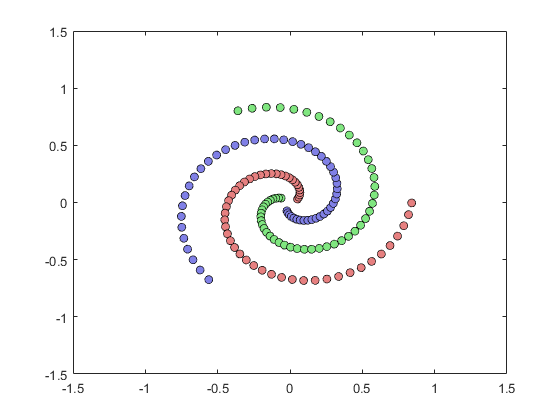
\includegraphics[width=\textwidth]{img/toy_spiral}
      \caption{Toy Spiral Data}
      \label{fig:toy_spiral}
    \end{subfigure}
    ~
    \begin{subfigure}{0.45\linewidth}
      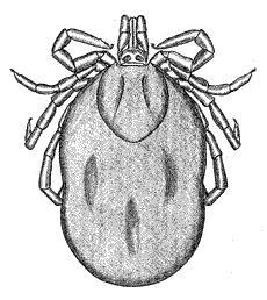
\includegraphics[width=\textwidth]{img/tick}
      \caption{Tick Image}
      \label{fig:tick_img}
    \end{subfigure}

	\caption{Examples of provided data sets.}
  \label{fig:example_data}
\end{figure}

The concepts of Randomised Decision Forest and K-means Codebook are well explained in the course notes, made available by Tae-Kyun Kim \cite{notes}. The authors assume that the reader is familiar with these concepts.


%-------------------------------------------------------------------------------
% Training Decision Forest
%-------------------------------------------------------------------------------
\section{Training Decision Forest}

The data used for this section is the Toy Spiral data, picture in Figure \ref{fig:toy_spiral}. One of the parameters which changes the way trees are grown in a RDF is the training data used to grow each tree; bagging (Bootstrap Aggregating) is used to split the training set up to provide random data sets from the same source.

\subsection{Bagging}

This process of bagging randomly selects a number of samples from a data set, with replacement. The size of the data sample is $100\% \times 1-e^{-1}=63.2\%$, which is common in machine learning; the effect of the data sample size is investigated in this report. Four examples of bagged data sets are shown in Figure \ref{fig:bagged_data}.

\begin{figure}[!ht]
  \captionsetup[subfigure]{position=b}
  \centering
    \begin{subfigure}{0.45\linewidth}
      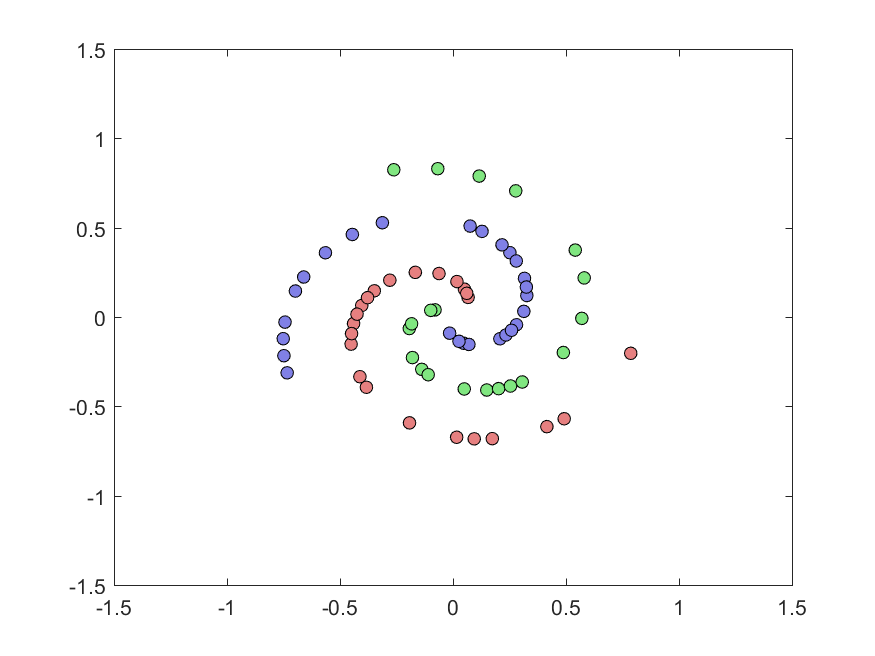
\includegraphics[width=\textwidth]{img/bagged_1}
      \caption{}
    \end{subfigure}
    ~
    \begin{subfigure}{0.45\linewidth}
      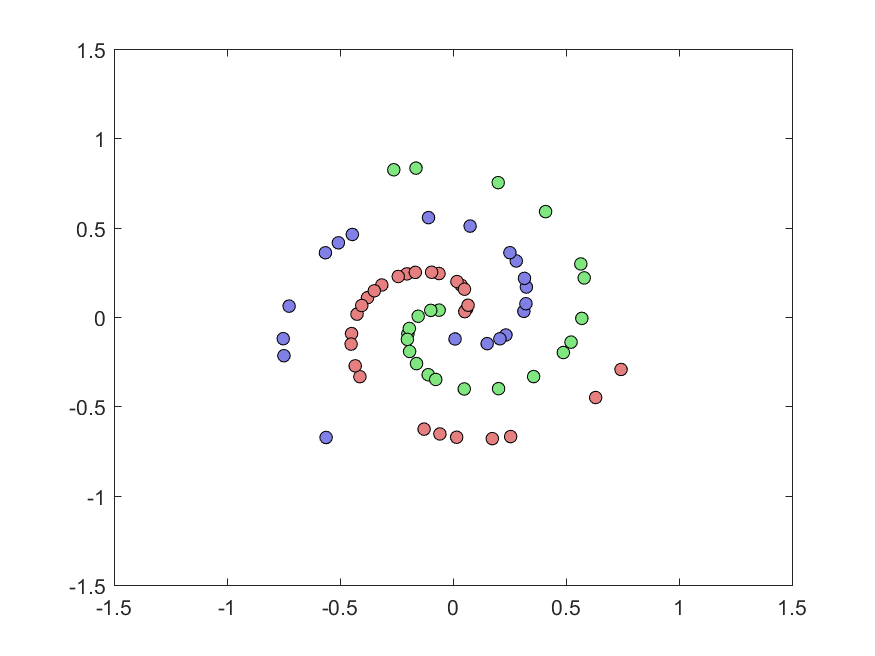
\includegraphics[width=\textwidth]{img/bagged_2}
      \caption{}
    \end{subfigure}
	\\
    \begin{subfigure}{0.45\linewidth}
      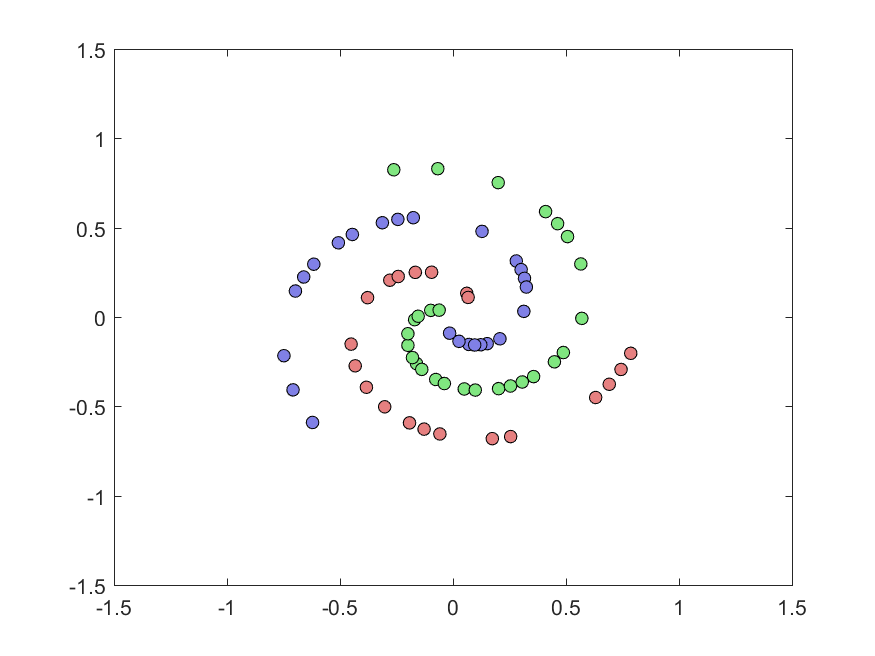
\includegraphics[width=\textwidth]{img/bagged_3}
      \caption{}
    \end{subfigure}
    ~
    \begin{subfigure}{0.45\linewidth}
      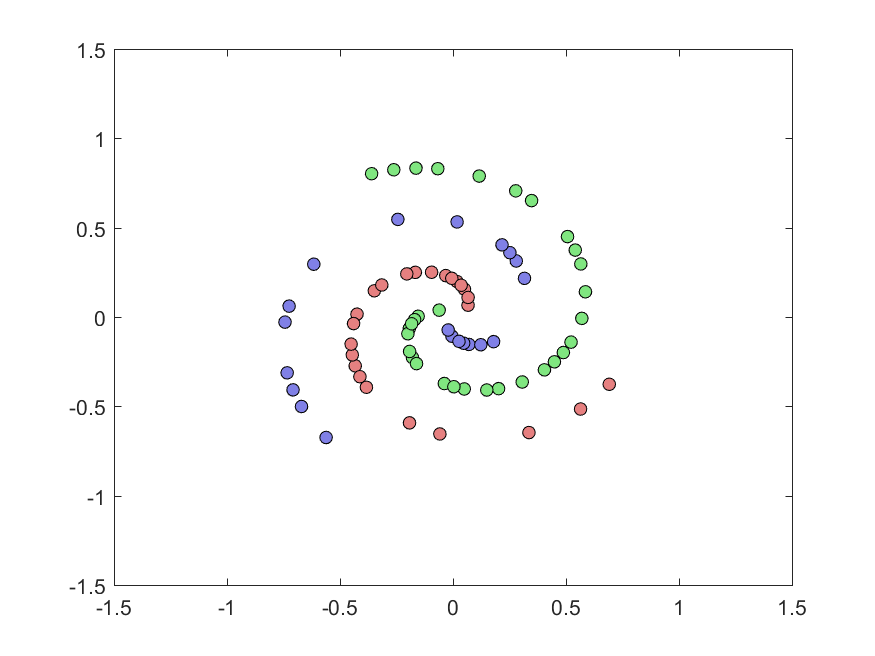
\includegraphics[width=\textwidth]{img/bagged_4}
      \caption{}
      \label{fig:used_bagged}
    \end{subfigure}

	\caption{(a):(d) Four bagged data sets.}
    \label{fig:bagged_data}
\end{figure}

\subsection{Investigating Decision Functions}

After the first sample was taken, the first tree could be grown from it. To test the split functions used in the process of growing the tree, various split functions were tested; although not shown here, axis-aligned performed as strongly as linear and quadratic with less computation time. The axis-aligned function was therefore used for subsequent tests. 

\subsection{Axis-Aligned Decision Function}

To investigate the axis-aligned function further, the parameter $\rho$ was varied, previously discussed as the number of splits. The complete range of $\rho=1,...n_{t}$ was attempted, where $n_t$ is the number of samples in the bagged data. The starting results are shown in Table \ref{tbl:axis_aligned_test}, as all results above $\rho=9$ had roughly the same information gain. As $\rho$ increases, the split function tends to become x-aligned with a threshold close to 0. The highest information gain is shown in Figure \ref{fig:best_axis}, with an x-aligned decision function with threshold -0.065988, with $\rho=60$. It is worth noting that the information gain shown by \texttt{splitNode.m} is slightly different from that later calculated due to rounding errors in the threshold.


\begin{table}[!ht]
	\centering
    \caption{Testing Axis-Aligned}
    \label{tbl:axis_aligned_test}
	\begin{tabular}{|lll|}
    	\hline
        \textbf{Splits Tested} & \textbf{IG} & \textbf{Time (s)} \\ \hline
        1 & -3.3151 & 0.25196 \\
        2 & -2.7972 & 0.14056  \\
        4 & -3.1663 & 0.11287  \\
        6 & -2.8237 & 0.11268  \\
        8 & -2.9141 & 0.11435  \\
        10 & -2.7715 & 0.11315 \\ \hline
	\end{tabular}
\end{table}

\begin{figure}[!ht]
  \centering
  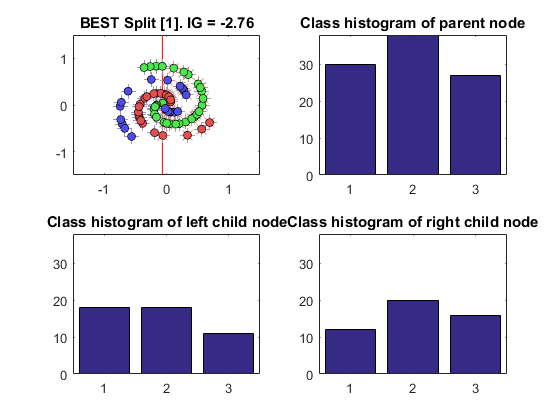
\includegraphics[width=\linewidth]{img/best_axis}
  \caption{Best information gain from axis-aligned decision function}
  \label{fig:best_axis}
\end{figure}

Given that the change in information gain is minimal above around $\rho=10$, $\rho$ is instead chosen based on the tend towards the x-aligned decision function, which peaks at around $\rho=50$. This value will be used to grow all subsequent trees.

\subsection{Tree Growth}

The node splitting was performed recursively, stopping at the maximum depth or if the node contained fewer than five samples; at this point, further splitting is inefficient. The class histograms of the first nine nodes are shown in Figure \ref{fig:leaf_vis}. 

Six out of nine of these histograms contain only one class in the leaf node, which is to be expected as it shows a successful split of the data; any data that is passed to this node is certain to be in the class provided. The remaining three leaf nodes contain only two classes, showing a strong probability of one class being correct, but a weak probability that a different one is correct. No leaf nodes shown have three classes, showing that the data is separable far enough to discern between classes. 

It may have been possible to end the algorithm when only one class is available per leaf node, but this could have caused an infinite loop if one data point sits exactly on top of another data point of a different class; furthermore, the tree could have been overfitted to the data set, reducing its ability to generalise.

The maximum depth used for the tree was eight, as this was found to give reasonable results in general testing. This parameter will be explored further in the next section. The maximum tree depth is the maximum depth of the tree before the data reaches a leaf node; as such, a larger depth can give more closely fitted results at the cost of generalisation.

\begin{figure}[!ht]
  \centering
  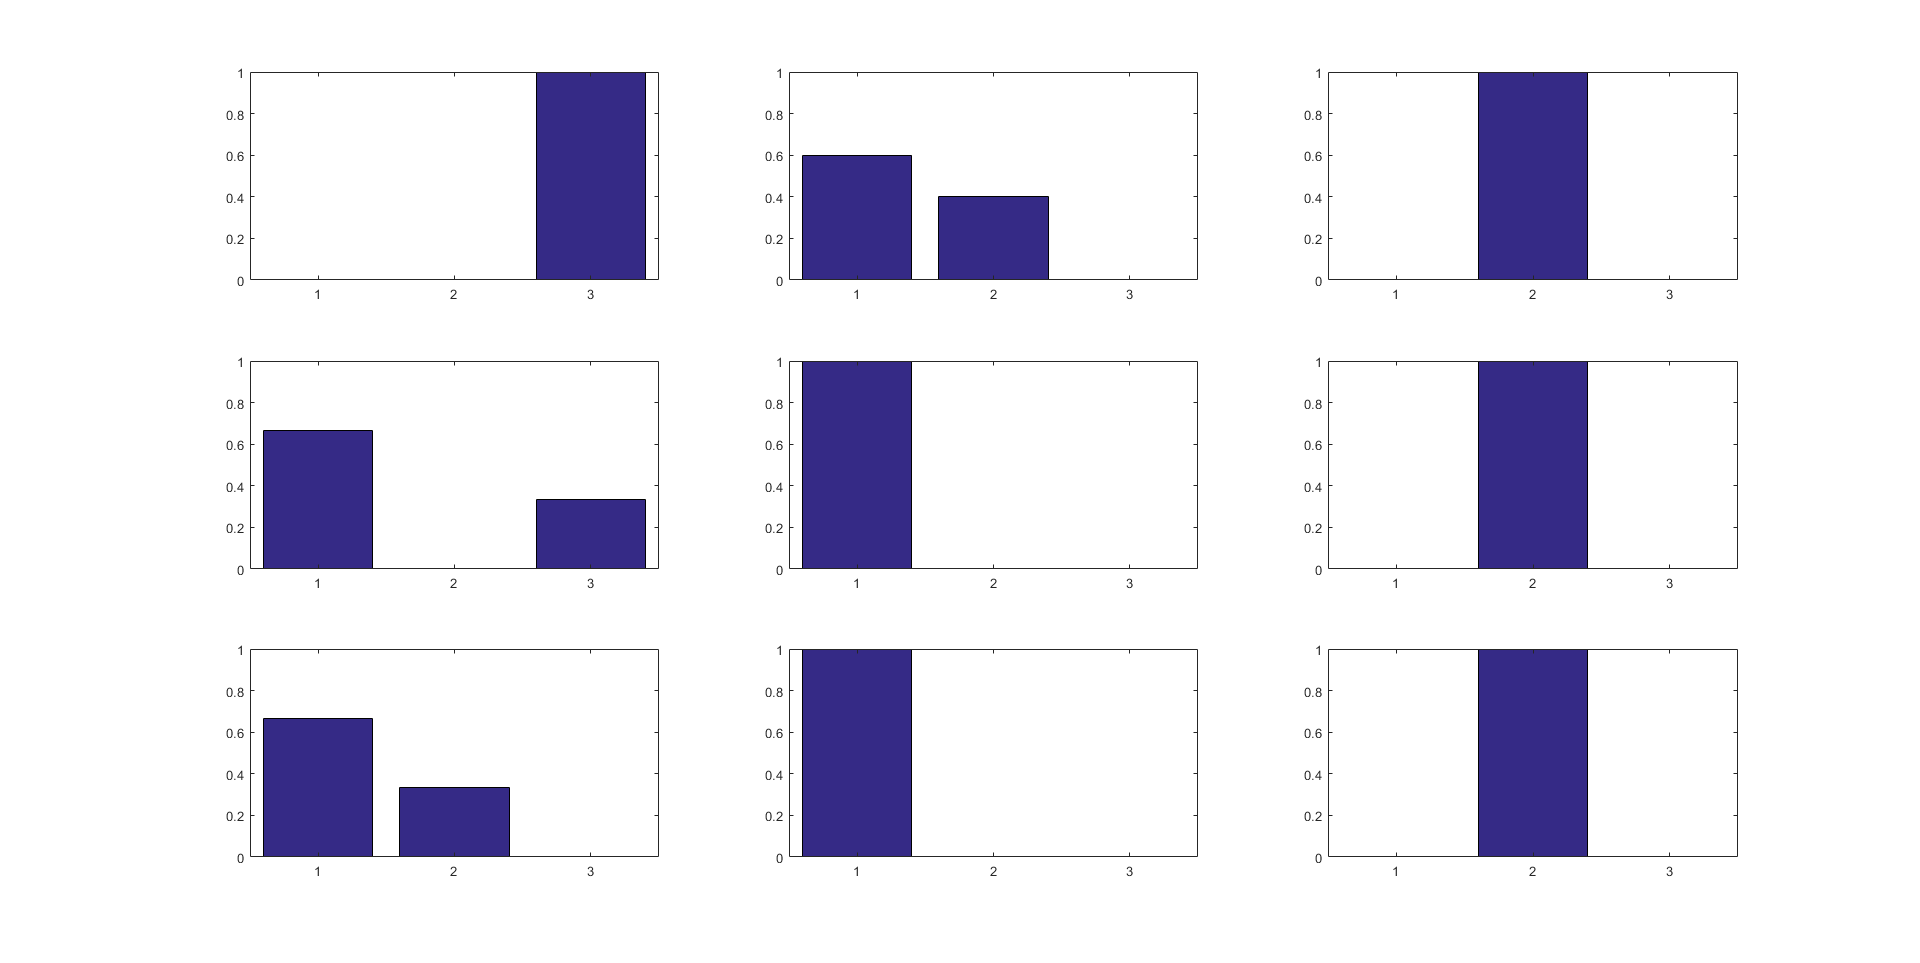
\includegraphics[width=\linewidth]{img/leaf_vis}
  \caption{Visualisation of 9 Leaf Nodes}
  \label{fig:leaf_vis}
\end{figure}


%-------------------------------------------------------------------------------
% Evaluating Decision Forest on the test data
%-------------------------------------------------------------------------------
\section{Evaluating Decision Forest on the test data}

\subsection{Forest Growth}

The previous topic covers the growth of an entire tree, but not the growth of a forest. The steps of the previous exercise are repeated for the same $\rho=50$, but with different bagged samples of data, to generate trees that are more independent of each other. In this way, the trees will produce different results, reducing the effect of overfitting; as a point can be tested on multiple trees in parallel, the computational efficiency of a single tree is kept when using a forest.

An RDF is grown using axis-aligned split functions, the same stopping criteria, and multiple bagged data sets, each of size 63.2\% of the original training data set. To evaluate how the tree identifies points, a number of test points are tested in the tree; for each point, the probabilities of the point being each class is output by each tree, which are then summed for all trees in the forest and divided by the number of trees to obtain a mean probability. The maximum probability is taken to be the leaf class.

The forest grown contained 5 trees, each with a maximum depth of 8, which is the number of splits allowed before classification is performed.

\subsection{Evaluate Test Points}

The test data points are as follows: [(-0.5, -0.7); (0.4, 0.3); (-0.7, 0.4); (0.5, -0.5)] \cite{instructions}. The results are shown in Figure \ref{fig:test_points}, where the four points can be seen as slightly outside the spiral, coloured by the class they are tested to be by the tree. The two points in blue and the point in red are clearly correct, and the point in green is between two spiral arms, making it difficult to classify; green is a reasonable guess given the arm to its right is also green. Therefore, all points have been classified successfully.

\begin{figure}[!ht]
  \centering
  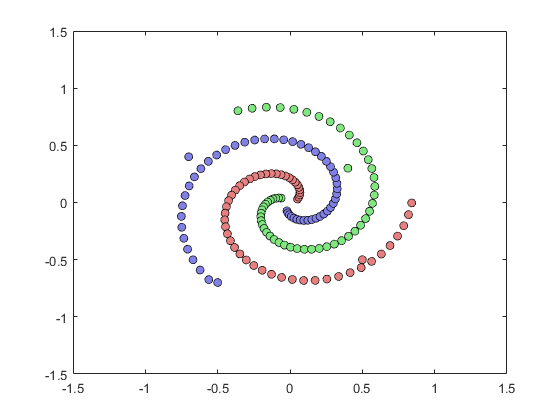
\includegraphics[width=\linewidth]{img/test_points}
  \caption{Spiral Data with Four Evaluated Test Points}
  \label{fig:test_points}
\end{figure}

\subsection{Evaluate Test Grid}

To visualise how the decision functions divide up the feature space, a dense grid of points was evaluated, provided in the given data as \texttt{data\_test}. Additionally, a more sparse grid of points is created and tested to allow the spiral data underneath to show through; this uses a grid of 50x50 across the feature space. The same forest from the previous section is evaluated for both grids, shown in Figure \ref{fig:grid_eval}.

\begin{figure}[!ht]
  \captionsetup[subfigure]{position=b}
  \centering
    \begin{subfigure}{0.45\linewidth}
      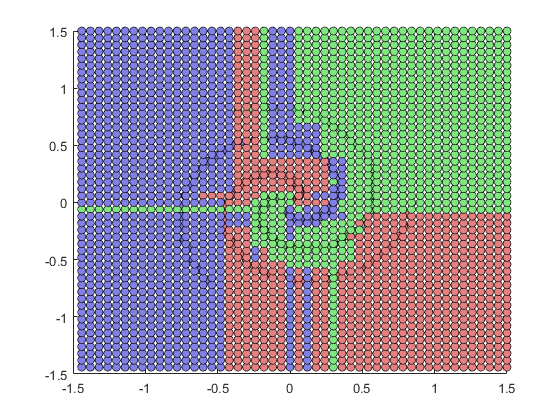
\includegraphics[width=\textwidth]{img/sparse_grid}
      \caption{Sparse Grid Evaluation}
      \label{fig:sparse_grid}
    \end{subfigure}
    ~
    \begin{subfigure}{0.45\linewidth}
      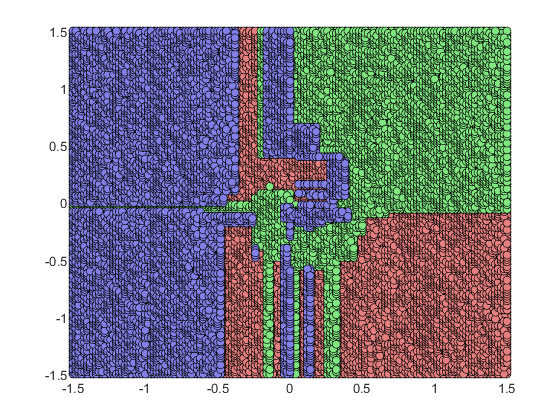
\includegraphics[width=\textwidth]{img/dense_grid}
      \caption{Dense Grid Evaluation}
      \label{fig:dense_grid}
    \end{subfigure}

  \caption{Result of evaluating test grids in Random Decision Forest using 5 trees with a maximum depth of 8 and axis-aligned decision functions}
  \label{fig:grid_eval}
\end{figure}

The results of the evaluation show clear rectangular sections corresponding to axis-aligned decision functions. The rectangles roughly overlay the spirals with the correct class, but do have breaks in the spirals where the forest misclassifies the data. There are large coloured sections outside the spiral edges where the decision functions never created a threshold, or the threshold clearly only contained one class.

\subsection{Varying Forest Parameters}

The RDF has different parameters that can affect its performance, including the split function. We continue to consider only the axis-aligned split function, but investigate the change in forest performance given a change in the number of trees, the maximum depth, the bagging fraction size, and the number of allowed splits. The tree is considered successful if it closely matches the spiral. Full results are not shown, but are referred to.
%The following investigation shows how two or more trees are required for good performance, how depth does not overly affect performance above a certain depth, how a high bagging fraction is required, and how very few attempted splits in a decision function can cause close fitting to the training data. The data shown is a small subset of the full data explored; as such, results discussed mainly pertain to the full set. 
All images are shown in the Appendix due to space requirements.

\subsubsection{Number of Trees}

The difference between just one and two trees in an RDF is shown in Figure \ref{fig:compare_no_trees}, where a single tree produces a single output for all evaluation points. A single decision tree would normally be overfitted to the data, but due to the randomness and depth restriction, it instead gives very poor results. One additional tree creates a far more effective forest, even though it is not the best performance possible. Further trees do improve performance, but a greater effect is seen from varying other parameters when two or more trees are used.


\subsubsection{Maximum Depth}

A shallow maximum depth gives a poor performance, giving only one output for the entire grid. At the opposite extreme, a very deep forest would be expected to provide overfitted data closely matching the spiral, but still has large blocks of incorrectly classified test points; this suggests that the other random parameters are sufficient to prevent the forest from overfitting.


\subsubsection{Number of Splits}

Although effect of the number of splits has been discussed for a single tree in a previous section, the effect of the number of splits on the forest overall has not been investigated. For a large number of splits, the forest seems to have much the same performance as before; for a small number, the forest has very high performance, with the test points closely matching the spiral. A small value of $\rho$ gives a high degree of randomness during data selection, and sufficiently many trees compensated for the reduced training data size per tree, giving overall high performance.

\subsubsection{Bagging Fraction}

The bagging fraction is the size of the bagged data as a fraction of the original training data set. A small fraction results in a very underfitted tree, with large portions of misclassified data, shown in Figure \ref{fig:sparse_6_8_25_1}. Figure \ref{fig:sparse_6_8_25_7} shows a better bagging fraction, with the forest fitting the data to the spiral much more closely, indicating better performance.

% Try different parameter values of RF and see the effects. RF has a few of important parameters,
% which need to be set to achieve good results. Here we try changing the number of trees, the depth
% of trees, and the degree of randomness parameter. Show and discuss the results for different
% parameter values.

% We've got pt1:
% treeNum = [1,2,4,6,8];
% treeDepth = [2, 4, 6, 8, 10,];
% treeSplits = 5:5:50;
% bagFracs = 0.1:0.2:1.0;



%-------------------------------------------------------------------------------
% Experiment with Caltech101 dataset for image categorisation
%-------------------------------------------------------------------------------
\section{Experiment with Caltech101 dataset for image categorisation}

The Caltech101 dataset contains images that fit into 10 classes. From each class, 15 images are randomly selected for the training and testing sets, each. The aim is to extract the features from the training images, which will then be used to create a visual ``codebook'' of features. Each image can be described in terms of the features (``codewords'') from the codebook. Representing an image in terms of the codewords is known as the vector quantisation process, which is explained in further detail below.

The \texttt{getData.m} function was first modified into the \texttt{getCaltechData.m} function, which contains just the section of the \texttt{getData.m} function that dealt with the \texttt{`Caltech'} argument, to simplify testing and experimentation. The \texttt{getCaltechData.m} function now returns 5 things.

\begin{itemize}
\item \texttt{desc\_tr} This is the collection of the features extracted from the training images.
\item \texttt{desc\_sel} This is the random selection from the training image features.
\item \texttt{desc\_te} These are the collection of the features extracted from the testing images.
\item \texttt{train\_index\_output} This are the indices of each training image.
\item \texttt{test\_index\_output} This are the indices of each testing image.
\end{itemize}

The entire code can be found in the Appendix.

\subsection{K-means Codewords}
In the script \texttt{q3\_1.m}, the K-means clustering was implemented using the \texttt{vl\_kmeans()} function which came with the \texttt{vlfeat-0.9.18} folder. The analysis of the intricacies of implementing a K-means method is not strictly the scope of the this report. However, it is worth mentioning that the reason for this function was that MATLAB's included \texttt{kmeans()} function was found to be unable to converge to a solution.

The input arguments to the \texttt{vl\_kmeans()} (Line 25 in \texttt{q3\_1.m}) were the selected features, along with the number of clusters. The distance type was the L2 one (the only other option was L1). Of note is the algorithm type, which was \texttt{ann}, as the function online description \cite{kmeans} suggested it as one suitable for large problems (with 100 000 points, it is safe to call this problem ``large'').

The only desired output was the list of centroid centres, which are used as the codewords in the codebook. Figure \ref{fig:visualcentroids} shows the list of centroids, represented as images, when 64 clusters are requested. The codewords are no longer visually meaningful, but still hold important information. The entire code for \texttt{q3\_1.m} is in the Appendix.

\begin{figure}[!ht]
    \centering
    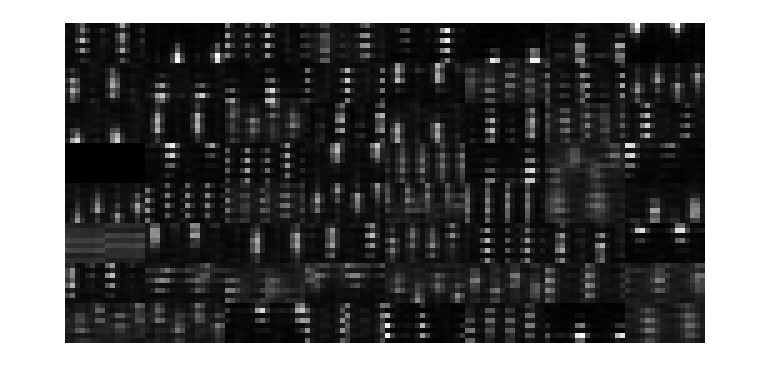
\includegraphics[width=.5\linewidth]{img/codewords64.png}
    \caption{Visualisation of codewords with $k =64$.}
    \label{fig:visualcentroids}
\end{figure}

\subsection{Vector Quantisation}
This takes the features from each picture and the codewords, and express how many of each codeword per picture there are, in the form of a histogram. The function \texttt{vec\_quant.m} does this. It cycles through each image of each class. Every feature is compared with all the codewords through the Nearest Neighbour (NN) method. The closest codeword to the feature is selected. At the end, the number of times each codeword is selected is collated and combined into a vector and displays the frequency of each one.

The only variation in this step is the type of distance metric used. While again, strictly not in the scope of this report, it is worth noting that the \texttt{nearest\_neighbour.m} function used implemented the L2 distance. It makes sense to have the method in the NN match that of the K-means clustering. Both \texttt{vec\_quant.m} and \texttt{nearest\_neighbour.m} are in the Appendix.

\subsection{Results}
In Figure \ref{fig:sameclass} are two training images from the same tick class. Both histograms from the training set have a sizable peak, but not at the same location. Looking at the other bins, there is not  much discernible. There is another histogram from the same tick class, but from the testing set. Comparing the testing histogram shows that there is again a peak (at yet another location), but the remaining bins are more ``noisy''. This could be the representation of the error between the training and testing sets. It is worth noting that like the codewords themselves, the histograms may not have meaningful visual representations, but hold value some other way.

\begin{figure}[!ht]
  \captionsetup[subfigure]{position=b}
  \centering
    \begin{subfigure}{0.45\linewidth}
      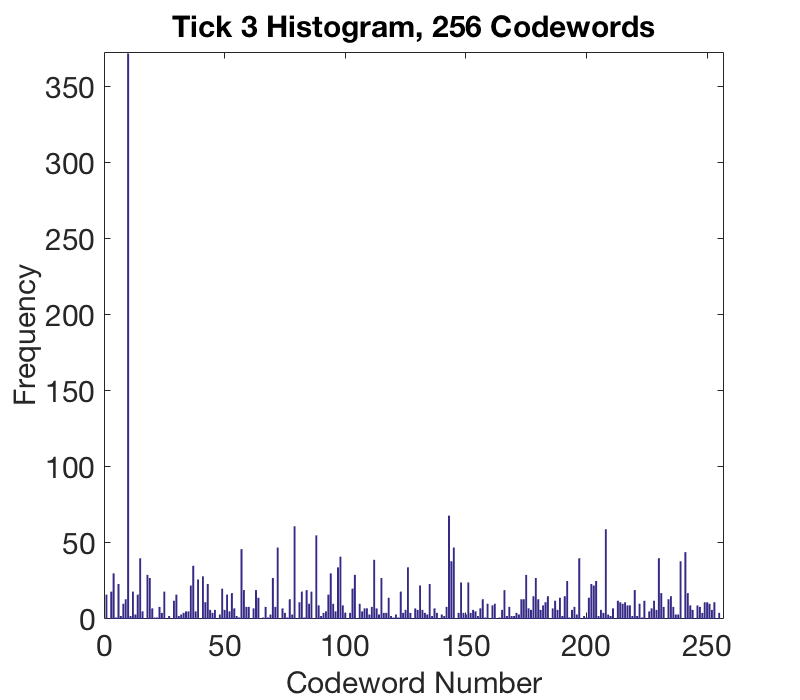
\includegraphics[width=\textwidth]{img/tick3_256}
      \caption{Histogram of Tick 3, 256 words.}
      \label{fig:sameclassb}
    \end{subfigure}
    ~
    \begin{subfigure}{0.45\linewidth}
      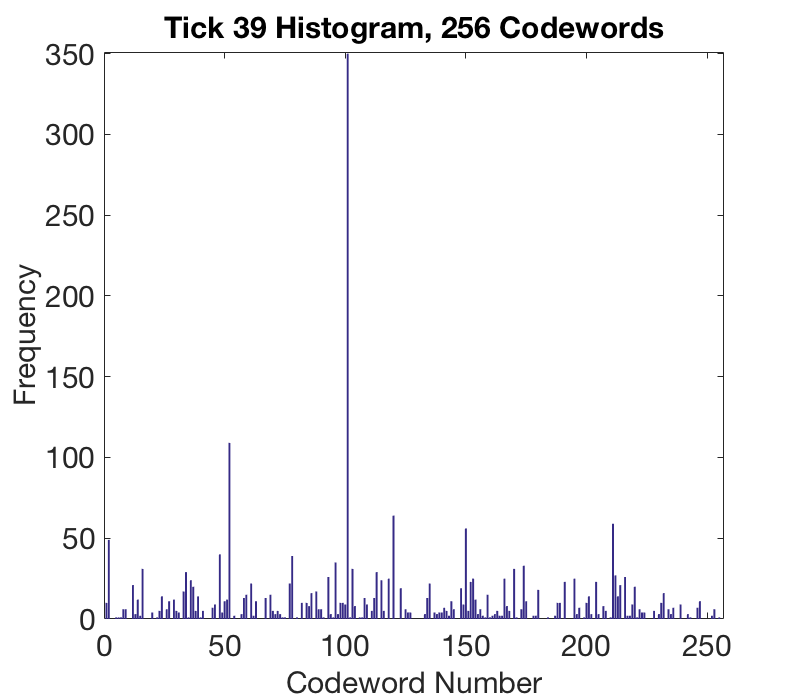
\includegraphics[width=\textwidth]{img/tick39_256}
      \caption{Histogram of Tick 39, 256 words.}
      \label{fig:sameclassd}
    \end{subfigure}
  	\\
    \begin{subfigure}{0.45\linewidth}
      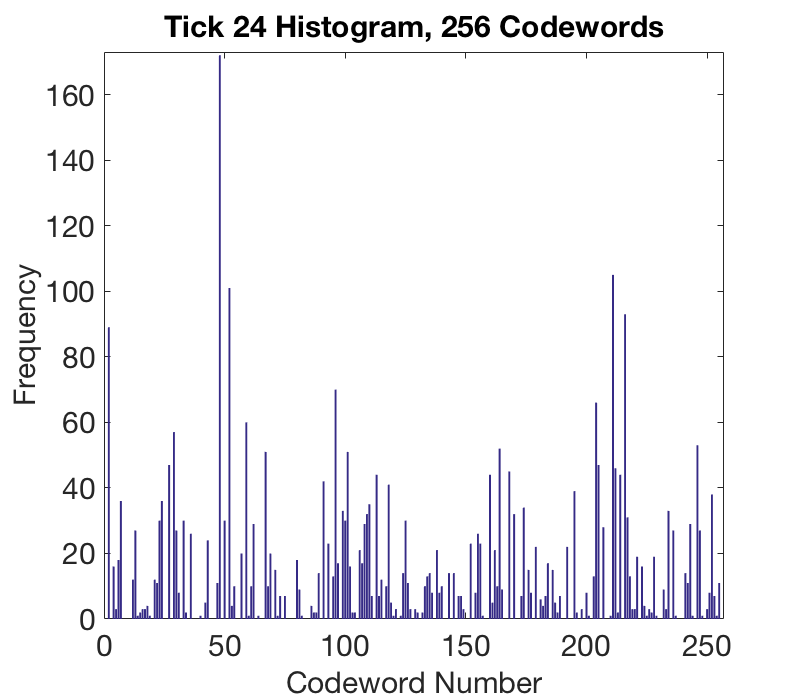
\includegraphics[width=\textwidth]{img/tick24_256}
      \caption{Histogram of Tick 24, 256 words.}
      \label{fig:sameclassf}
    \end{subfigure}

  \caption{Same class images and their histograms}
  \label{fig:sameclass}
\end{figure}

In Figure \ref{fig:diffclass}, there are three histograms, each from a different class in the training set. Their histograms are very different from each other, both in peaks and spread. This suggests that there is enough information contained to achieve effective classification.

\begin{figure}[!ht]
  \captionsetup[subfigure]{position=b}
  \centering
    \begin{subfigure}{0.45\linewidth}
      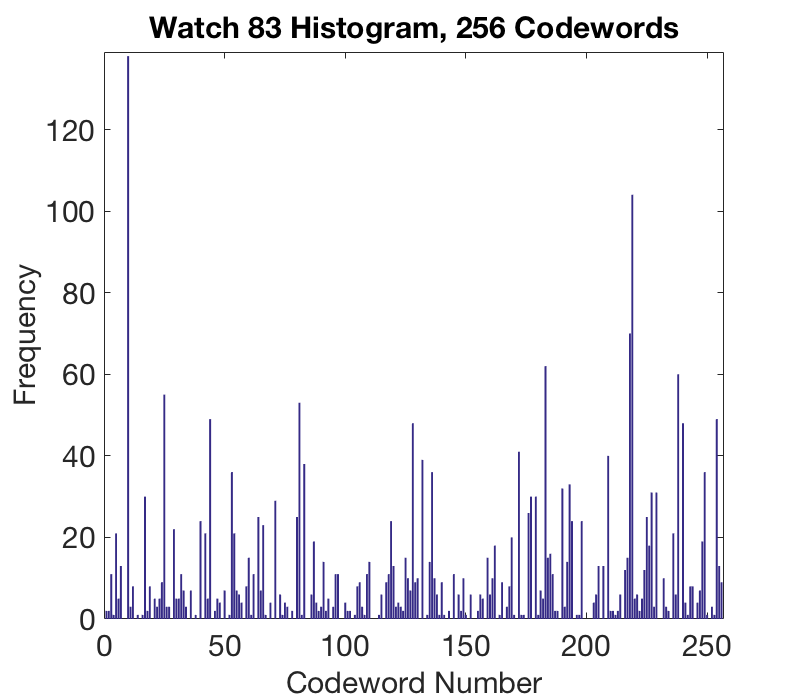
\includegraphics[width=\textwidth]{img/watch83_256}
      \caption{Histogram of Watch 83, 256 words.}
      \label{fig:diffclassb}
    \end{subfigure}
    ~
    \begin{subfigure}{0.45\linewidth}
      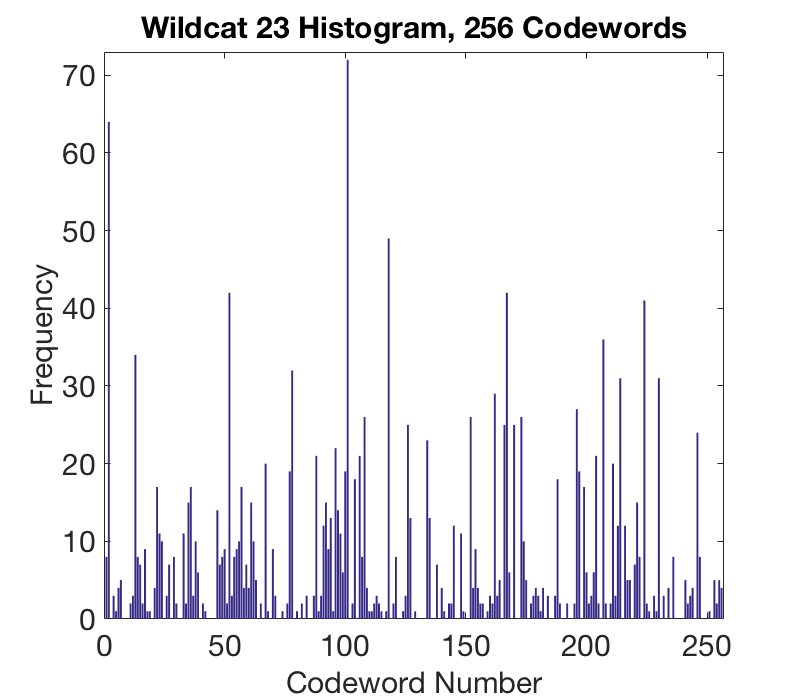
\includegraphics[width=\textwidth]{img/wildcat23_256}
      \caption{Histogram of Wildcat 23, 256 words.}
      \label{fig:diffclassd}
    \end{subfigure}
    \\
    \begin{subfigure}{0.45\linewidth}
      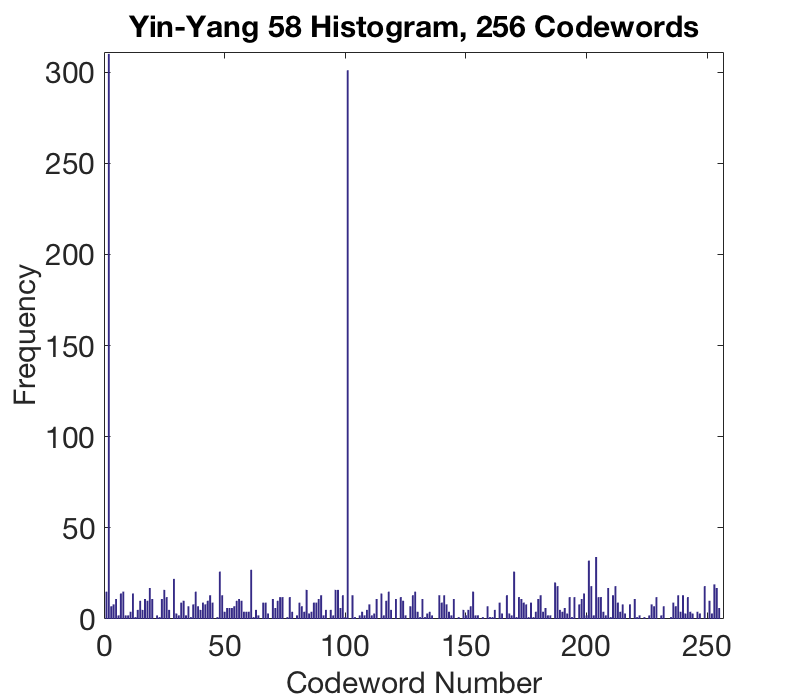
\includegraphics[width=\textwidth]{img/yy58_256}
      \caption{Histogram of Yin-Yang 58, 256 words.}
      \label{fig:diffclassf}
    \end{subfigure}

  \caption{Different class images and their histograms}
  \label{fig:diffclass}
\end{figure}

The other parameter that can be varied is the size of the codebook. The process was repeated for $k \in \left\{ 64, 128, 256, 512 \right\}$. To allow an accurate comparison, the same Tick 3 of Figure \ref{fig:sameclass} is used, but the histograms with 4 different sized codebooks are shown instead in Figure \ref{fig:diffk}. When $k \in \left\{ 64, 128, 256 \right\}$, each histogram displays a significant peak somewhere, while this is not the case when $k =512 $. The location of the peak itself is difficult to make meaningful as the arbitrary naming of the clusters in the function means that the strict ``order'' is not important. Another thing to note is the time spent on the clustering and quantisation. The times in seconds are 96.01, 118.78, 114.79, and 117.81 from the function output, but 70.6594, 106.5945, 129.6862, and 180.6909 from the MATLAB timing. 

\begin{figure}[!ht]
  \captionsetup[subfigure]{position=b}
  \centering
    \begin{subfigure}{0.45\linewidth}
      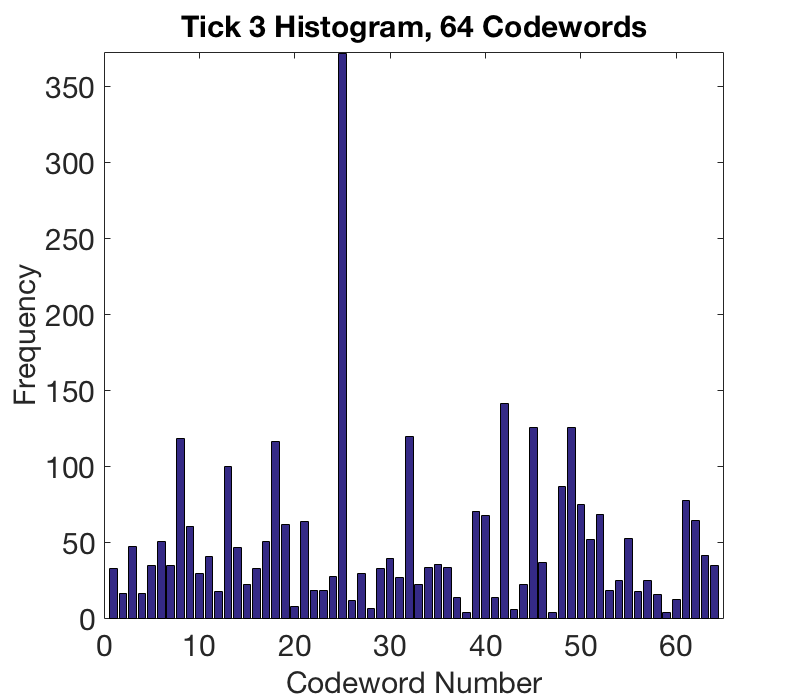
\includegraphics[width=\textwidth]{img/tick3_64}
      \caption{$k = 64$}
      \label{fig:diffk64}
    \end{subfigure}
    ~
    \begin{subfigure}{0.45\linewidth}
      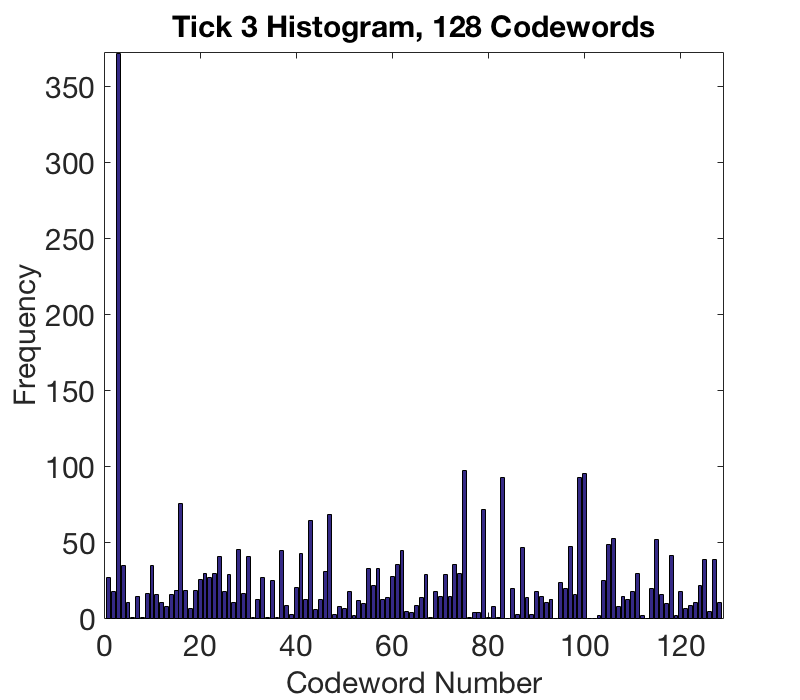
\includegraphics[width=\textwidth]{img/tick3_128}
      \caption{$k = 128$}
      \label{fig:diff128}
    \end{subfigure}
    \\
    \begin{subfigure}{0.45\linewidth}
      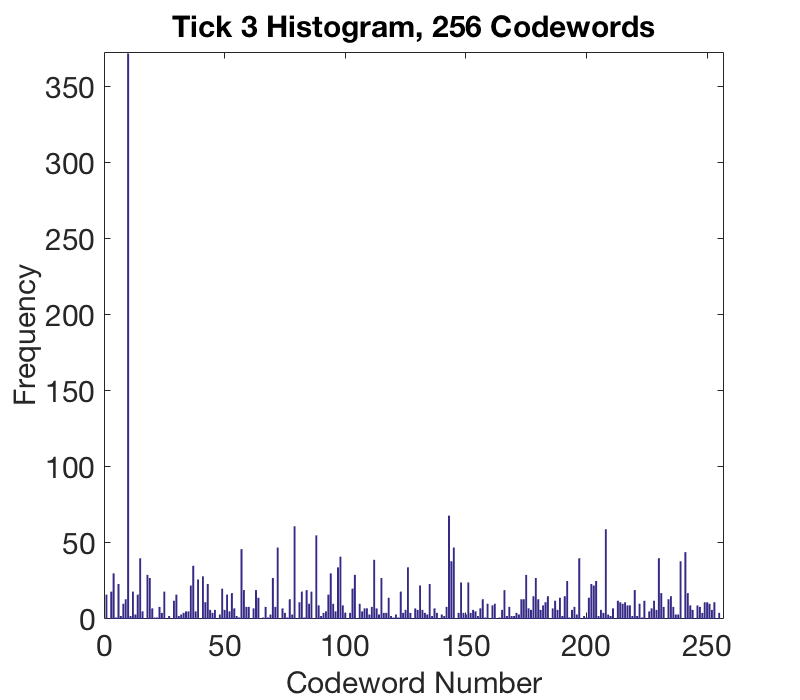
\includegraphics[width=\textwidth]{img/tick3_256}
      \caption{$k = 256$}
      \label{fig:diff256}
    \end{subfigure}
    ~
    \begin{subfigure}{0.45\linewidth}
      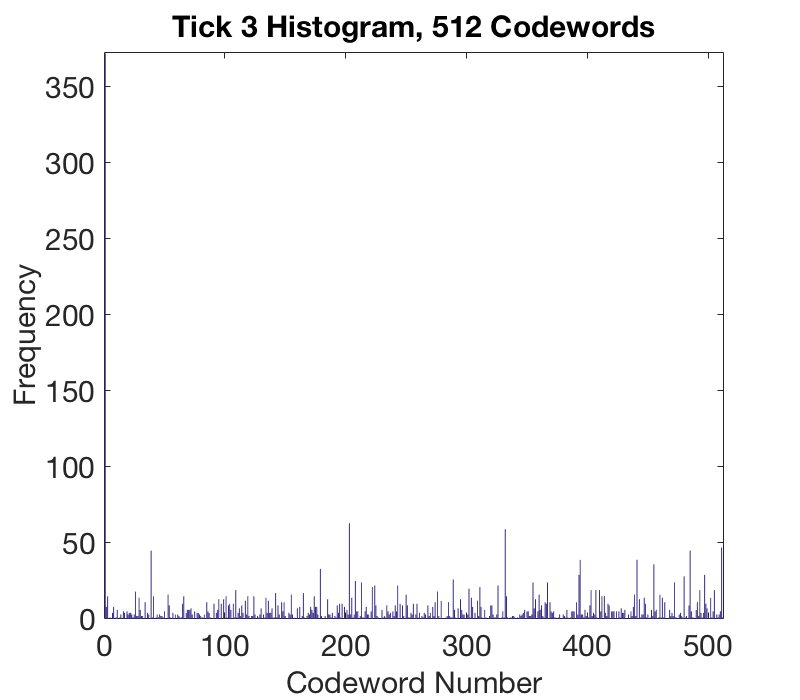
\includegraphics[width=\textwidth]{img/tick3_512}
      \caption{$k = 512$}
      \label{fig:diffk512}
    \end{subfigure}

  \caption{Same Tick 3 histograms, different $k$.}
  \label{fig:diffk}
\end{figure}

\section{RF Classifier}
Using the histograms, the images can be classified using an RF. Each image is now treated through its histogram, meaning that is a vector composed of the frequency of each codeword. These are fed into the RF generation function together with the associated class.

Each testing image, which has already been quantised into a vector using the same codebook, is fed through the RF. And as previously, the leaf node where it ends up in each tree has an associated distribution for the training classes. This is combined to obtain the final class decision. The code for the RF classifier is in the Appendix.

\subsection{Sample Results}
Taking the training data that was quantised with the 256-word codebook as starting point, the RF was trained. Then the training data was fed through, and analysed. The initial parameters were 3 trees, 13 node depth, 50 split functions, and and axis-aligned decision function. The confusion matrix is shown in Figure \ref{fig:rfclassifier}.
\begin{figure}[H]
    \centering
    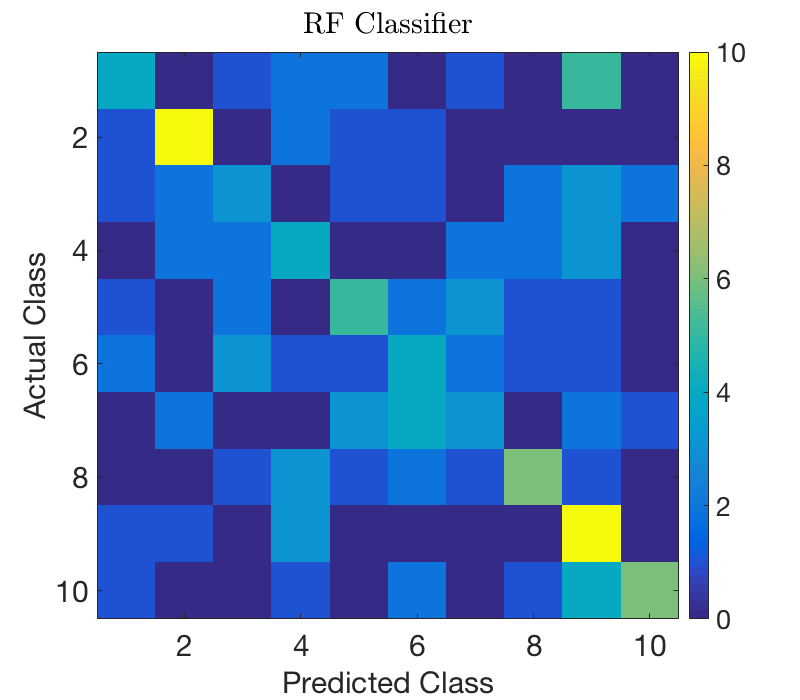
\includegraphics[width=0.45\linewidth]{img/rfclassifier}
    \caption{Confusion Matrix with initial parameters, $k = 256$.}
    \label{fig:rfclassifier}
\end{figure}
This is not particular good. In fact, the classification accuracy overall was only 36.6667\%. However, it worth noting that the classifier did very well for certain classes, which were 2 and 9. Those were the trilobite and wrench classes. The impact of the different parameters to improve accuracy can be further investigated.

\subsection{Varying Forest Parameters}

To test the performance of the classifier, the random forest parameters and the size of K were varied to test the difference in classification accuracy. The full set of results is too large to display; Table \ref{tbl:rf_discussed} gives the subset of result discussed in the following sections. The train times overall were found to increase with the number of nodes per forest and the size of K, whereas the test times stayed mostly constant between 10 and 50ms. Furthermore, the size of K was found to have little effect on the accuracy of the classification, shown in the table as 44\% and 43\% success rates for $K=64$ and $K=512$ respectively; this lack of trend continued through the rest of the data.

\begin{table}[!ht]
  \centering
  \caption{Discussed Results in RF Classifier}
  \label{tbl:rf_discussed}
  \begin{tabular}{|lllllll|}
  	\hline
    K & Trees & Depth & Rho & Accuracy & Train (s) & Test (s) \\ \hline
    64  & 6 & 10 & 25 & 44.00 & 1.21 & 0.041 \\
    512 & 6 & 10 & 25 & 43.33 & 2.50 & 0.039 \\
    256 & 1 & 10 & 25 & 10.00 & 0.31 & 0.011 \\
    256 & 8 & 10 & 25 & 40.67 & 2.09 & 0.049 \\
    256 & 6 & 2  & 25 & 19.33 & 0.17 & 0.018 \\
    256 & 6 & 10 & 25 & 37.33 & 1.70 & 0.038 \\
    256 & 6 & 10 & 2  & 42.67 & 1.66 & 0.034 \\
    256 & 6 & 10 & 50 & 33.33 & 1.56 & 0.039 \\
    64  & 6 & 8  & 2  & 51.33 & 1.09 & 0.041 \\
  \hline
\end{tabular}

\end{table}

A single tree in a forest gives a highly inaccurate result, showing the lowest accuracy over the whole data set. However, two or more trees give similar performance, with more trees giving slightly higher performance. Naturally, this increase in trees in conjunction with other parameters has more of an effect on the classification result. A shallow tree depth gave a poor performance, with a result of 19.33\% in the table, compared to a depth of 10 with the same parameters giving 37\% accuracy. However, as with the number of trees, a higher depth generally gives better performance, but other parameters have more of an effect.

The number of split functions allowed directly corresponds to the randomness parameter $\rho$. In this set of tests, a very low value of $\rho$ showed strong performance due to the high degree of randomness, where $\rho = 2$ had an accuracy of 43\% for $K=256$, and the overall highest accuracy of 51\% with other parameter changes. As the number of splits increased to 50, the accuracy decreased back to 33\%, showing that the number of splits plays a very strong role in the ability of the forest to classify data.

Maximising the classification error was placed at a lower priority than exploring the impact of different parameters as higher accuracy rates could be too computationally intensive.

\section{RF Codebook}
Instead of using K-means to create a codebook from the randomly selected features, another way is to feed the features from all the data in the training set directly into the RF generator. After the trees have all been generated, the features from each image are passed through the forest for quantisation, and classification.

\subsection{RF Generation Observations}
The most important was the training time. The RF codeword generation was faster than with the K-means codewords. According to the notes \cite{notes}, this is expected as the complexity of training with K-means is $\mathcal{O}(DNK)$, where $D$ is the dimension of the features, $N$ is the number of patches, and $K$ is the number of clusters. This is contrast to the RF method, which is $\mathcal{O}(\sqrt{D}N\log{K})$, where $K$ is the number of leaves.

The size of codebook was dictated by the number of trees created, and how many leaf nodes they would end up with, and in this case means that this method has one advantage for large codebooks.

\subsection{Vector Quantisation}
Each image will have each of its features passed through the forest. Each feature ends up at a leaf node for each tree. Across all the trees, treating each leaf node as separate, each image with its features landing with some distribution over all the leaf nodes. These numbers of features per leaf node are then used to produce a histogram, just like the K-means method.

\subsection{Classification}
Like in the previous case with the K-means codebook, an RF was used. In other words, after the codebook in this section was generated using RF instead of K-means, the same RF method was used to classify the resultant histograms. To keep things simple, as the effects of the classification RF parameters were already observed, a classification RF with 8 trees and a depth of 10 was used.

\subsection{Results}
The notes point to the size of the codebook as an important factor, which is a function of the depth and tree number. As such, the same data was run through the RF codebook creation step with different tree numbers and depths. The entire set of confusion matrices can be seen in the Appendix, but the results, such as classification accuracy and time are included in Table \ref{tbl:rfrf}.

\begin{table}[!ht]
  \centering
  \caption{Discussed Results in RF Classifier}
  \label{tbl:rfrf}
  \begin{tabular}{|llll|}
  	\hline
    Trees & Depth & Accuracy & Time for RF \\ \hline
    2 & 2 & 38.67\% & 6.84\\
    2 & 6 & 46\% & 31.6547\\
    6 & 2 & 32\% & 20.7297\\
    6 & 6 & 40\% & 102.65\\
  \hline
\end{tabular}

The reason for the few results is that while the time to create the RF codebook was relatively short, the time required to quantise every image took much longer, almost prohibitively long for the larger depth and tree selections. Realistically, it was not possible without setting aside many days. The quantisation for K-means is much shorter, even through the RF codebook generation was quicker. Accuracy improvements from this limited data set is difficult to say, however, it would appear that the depth of each tree plays a bigger role than the number of trees when it comes to RF codebook generation and the resultant classification accuracy. 

\end{table}


%-------------------------------------------------------------------------------
% Conclusion
%-------------------------------------------------------------------------------
\section{Conclusion}

This paper first considered the use of Random Decision Forests (RDFs) as classifiers for two dimensional labelled data, finding that given a sufficiently large forest, further increases to the number of trees or depth of each tree does not affect the forest much. Furthermore, a high level of randomness was found to perform better, but only given a sufficiently large forest to compensate; a large, highly random forest performed best, as expected.

K-means codebook was used to create a set of codewords describing image sets, which was then classified using an RDF. Results were poor, with at most 51\% accuracy, and larger numbers of clusters above 64 having little effect except for increased training time. 

For the RDF generated codebook, it was a much quicker method. However, in practice, the quantisation of the training and test sets took much longer, and was long enough that it made true exploration difficult. That being said, more trees and depth gave better accuracy overall.

%-------------------------------------------------------------------------------
% References
%-------------------------------------------------------------------------------
\bibliographystyle{unsrt}
\bibliography{mlcv_refs}

%-------------------------------------------------------------------------------
% Appendix(ces)
%-------------------------------------------------------------------------------
\onecolumn
\section*{Appendix}

\subsection*{Forest Parameter Variation Images}
\begin{figure}[!ht]
  \captionsetup[subfigure]{position=b}
  \centering
    \begin{subfigure}{0.45\linewidth}
      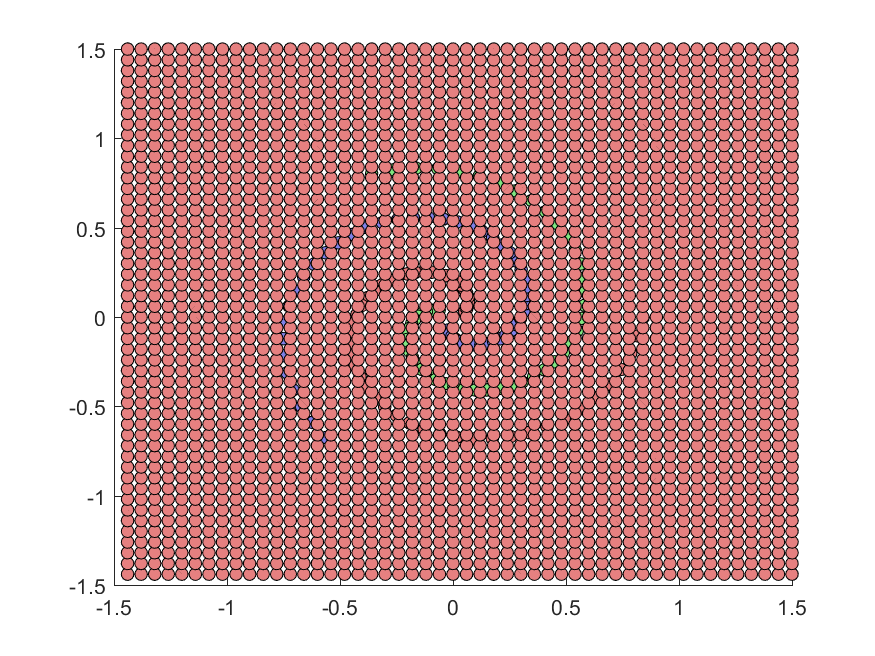
\includegraphics[width=\textwidth]{img/tree_params/tree_sparse_1_10_50_7}
      \caption{Sparse Evaluation on RDF with 1 tree, 10 depth, 50 splits, and 0.7 bagging fraction}
      \label{fig:sparse_1_10_50_7}
    \end{subfigure}
    ~
    \begin{subfigure}{0.45\linewidth}
      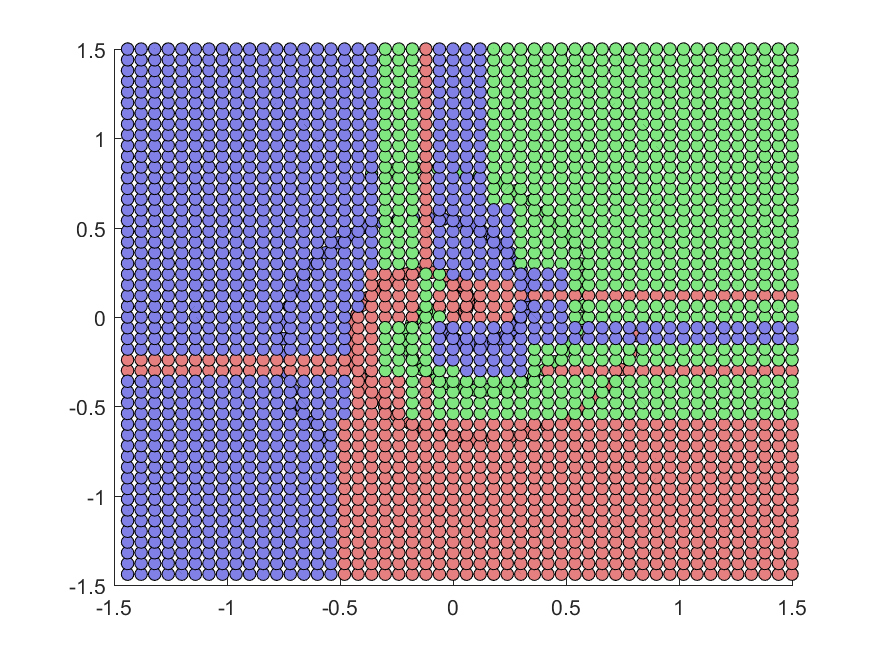
\includegraphics[width=\textwidth]{img/tree_params/tree_sparse_2_10_50_7}
      \caption{Sparse Evaluation on RDF with 2 trees, 10 depth, 50 splits, and 0.7 bagging fraction}
      \label{fig:sparse_2_10_50_7}
    \end{subfigure}

  \caption{Comparison of effect of number of trees in RDF}
  \label{fig:compare_no_trees}
\end{figure}

\begin{figure}[!ht]
  \captionsetup[subfigure]{position=b}
  \centering
    \begin{subfigure}{0.45\linewidth}
      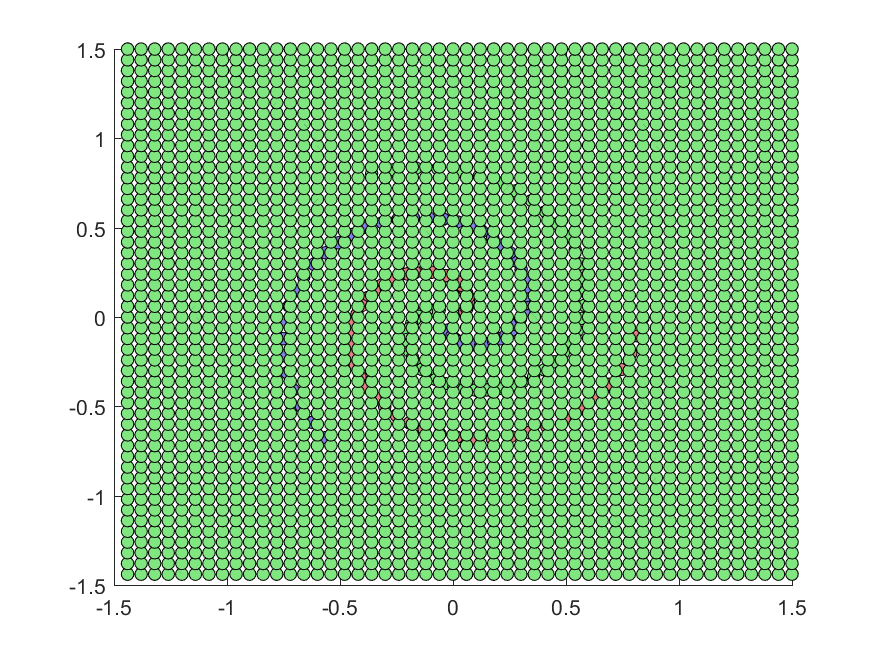
\includegraphics[width=\textwidth]{img/tree_params/tree_sparse_6_2_50_7}
      \caption{Sparse Evaluation on RDF with 6 trees, 2 depth, 50 splits, and 0.7 bagging fraction}
      \label{fig:sparse_6_2_50_7}
    \end{subfigure}
    ~
    \begin{subfigure}{0.45\linewidth}
      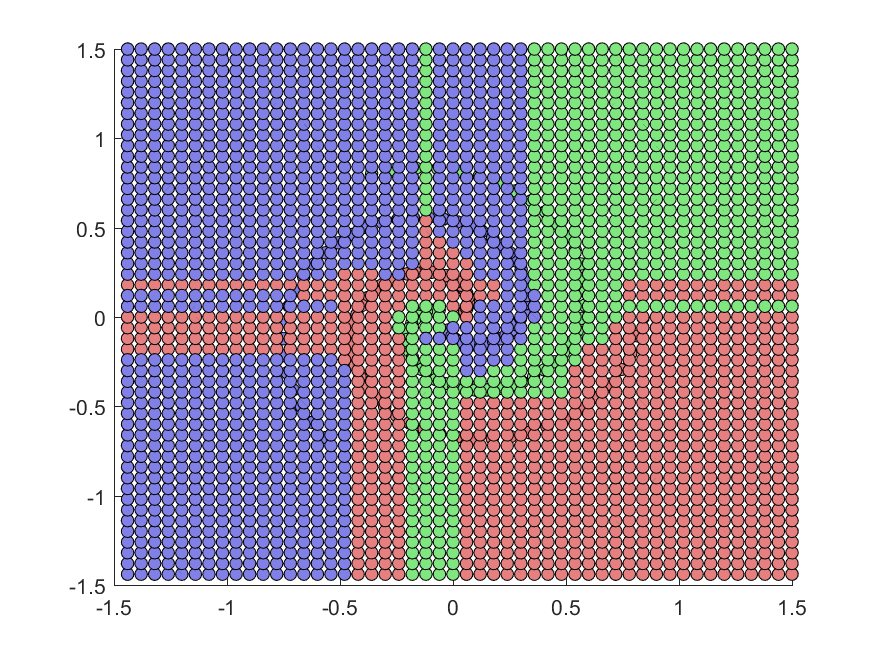
\includegraphics[width=\textwidth]{img/tree_params/tree_sparse_6_14_50_7}
      \caption{Sparse Evaluation on RDF with 6 trees, 14 depth, 50 splits, and 0.7 bagging fraction}
      \label{fig:sparse_6_14_50_7}
    \end{subfigure}

  \caption{Comparison of effect of maximum depth in RDF}
  \label{fig:compare_depth}
\end{figure}

\begin{figure}[!ht]
  \captionsetup[subfigure]{position=b}
  \centering
    \begin{subfigure}{0.45\linewidth}
      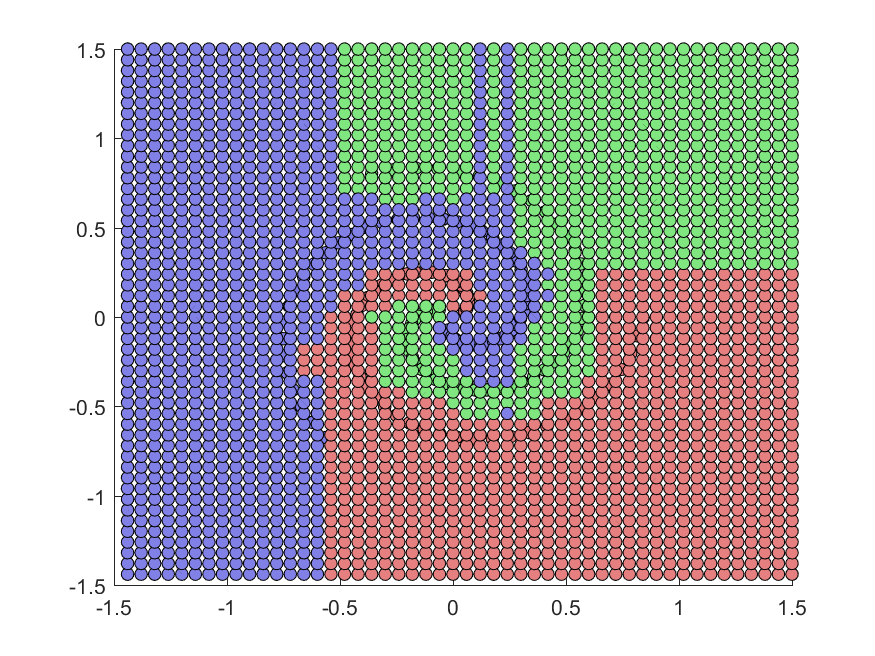
\includegraphics[width=\textwidth]{img/tree_params/tree_sparse_6_8_2_7}
      \caption{Sparse Evaluation on RDF with 6 trees, 8 depth, 2 splits, and 0.7 bagging fraction}
      \label{fig:sparse_6_8_2_7}
    \end{subfigure}
    ~
    \begin{subfigure}{0.45\linewidth}
      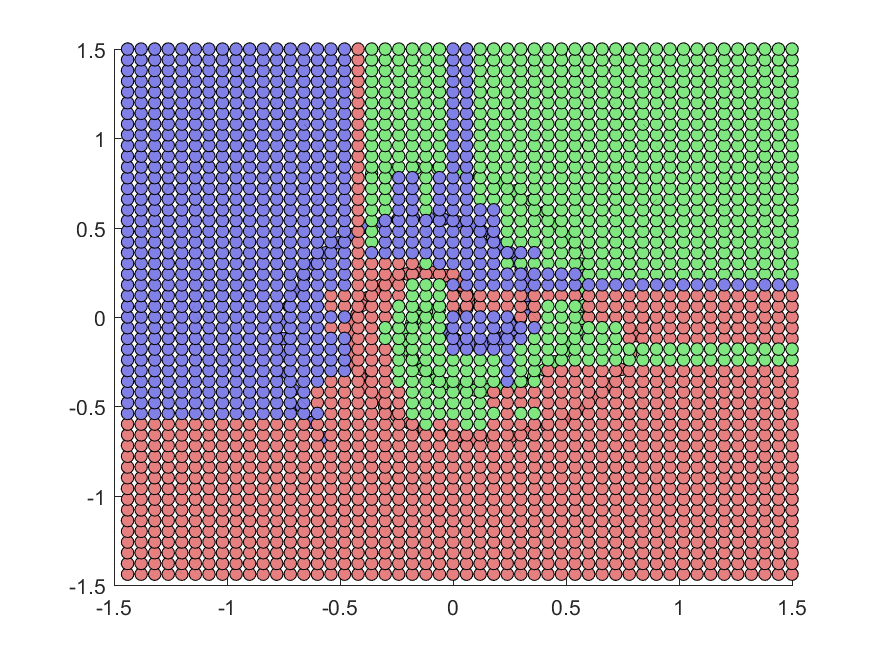
\includegraphics[width=\textwidth]{img/tree_params/tree_sparse_6_8_50_7}
      \caption{Sparse Evaluation on RDF with 6 trees, 8 depth, 50 splits, and 0.7 bagging fraction}
      \label{fig:sparse_6_8_50_7}
    \end{subfigure}

  \caption{Comparison of effect of number of splits in RDF}
  \label{fig:compare_splits}
\end{figure}


\begin{figure}[!ht]
  \captionsetup[subfigure]{position=b}
  \centering
    \begin{subfigure}{0.45\linewidth}
      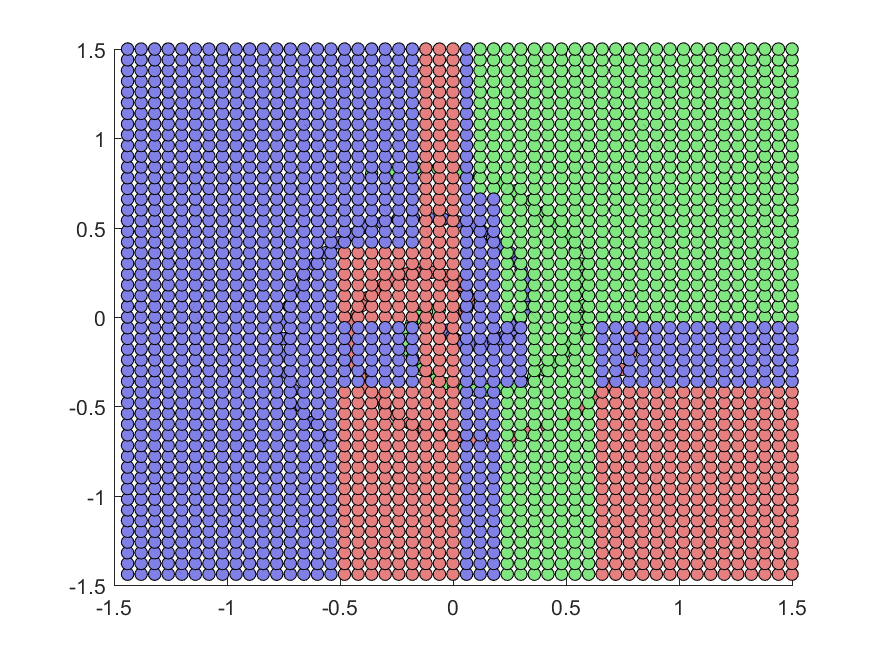
\includegraphics[width=\textwidth]{img/tree_params/tree_sparse_6_8_25_1}
      \caption{Sparse Evaluation on RDF with 6 trees, 8 depth, 25 splits, and 0.1 bagging fraction}
      \label{fig:sparse_6_8_25_1}
    \end{subfigure}
    ~
    \begin{subfigure}{0.45\linewidth}
      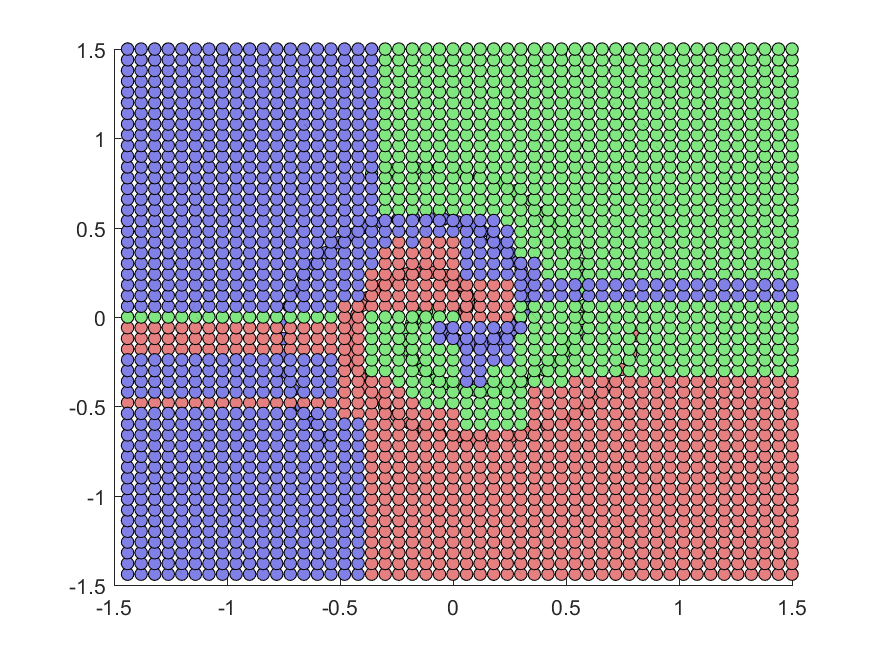
\includegraphics[width=\textwidth]{img/tree_params/tree_sparse_6_8_25_7}
      \caption{Sparse Evaluation on RDF with 6 trees, 8 depth, 25 splits, and 0.7 bagging fraction}
      \label{fig:sparse_6_8_25_7}
    \end{subfigure}

  \caption{Comparison of effect of bagging fraction in RDF}
  \label{fig:compare_bagging}
\end{figure}

\subsection*{texttt{getCalTechData.m} Function}
\lstinputlisting[style=Matlab-editor]{src/getCalTechData.m}
\newpage

\subsection*{texttt{q1\_3} Function, Featuring K-means}
\lstinputlisting[style=Matlab-editor]{src/q3_1.m}
\newpage

\subsection*{Vector Quantisation Function}
\lstinputlisting[style=Matlab-editor]{src/vec_quant.m}

\subsection*{Nearest Neighbour Function}
\lstinputlisting[style=Matlab-editor]{src/nearest_neighbour.m}
\newpage

\subsection*{Histogram Output Function}
\lstinputlisting[style=Matlab-editor]{src/histogramoutput.m}

\subsection*{RF Classifier Code}
\lstinputlisting[style=Matlab-editor]{src/rfclass.m}
\newpage

\subsection*{RF Codebook Code}
\lstinputlisting[style=Matlab-editor]{src/q3_3c.m}
\newpage

\subsection*{RF Quantisation Code}
\lstinputlisting[style=Matlab-editor]{src/rf_histogram.m}
\newpage

\subsection*{RF Confusion Matrices}
\begin{figure}[!ht]
  \captionsetup[subfigure]{position=b}
  \centering
    \begin{subfigure}{0.45\linewidth}
      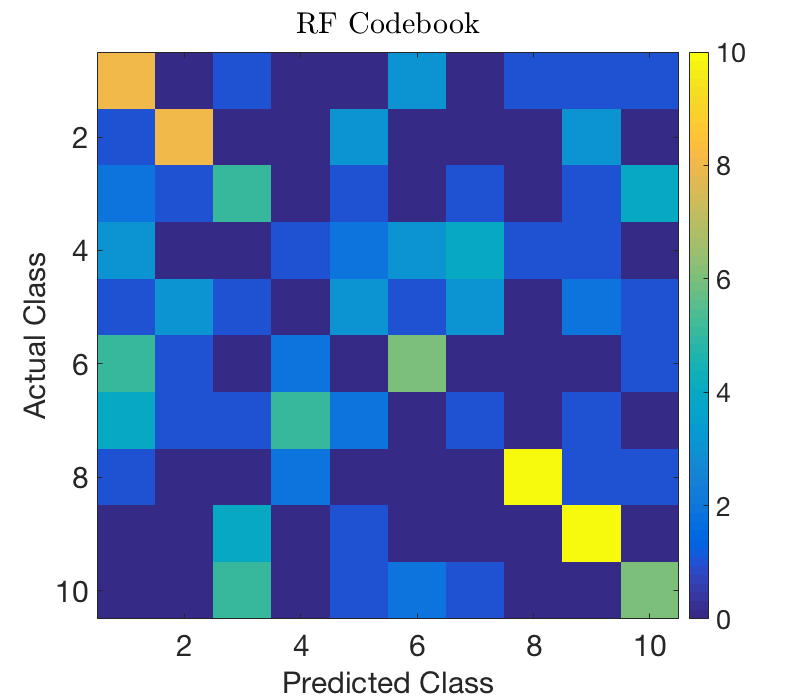
\includegraphics[width=\textwidth]{img/rfrf22}
      \caption{2 trees, depth 2.}
      \label{fig:rfrf1}
    \end{subfigure}
    ~
    \begin{subfigure}{0.45\linewidth}
      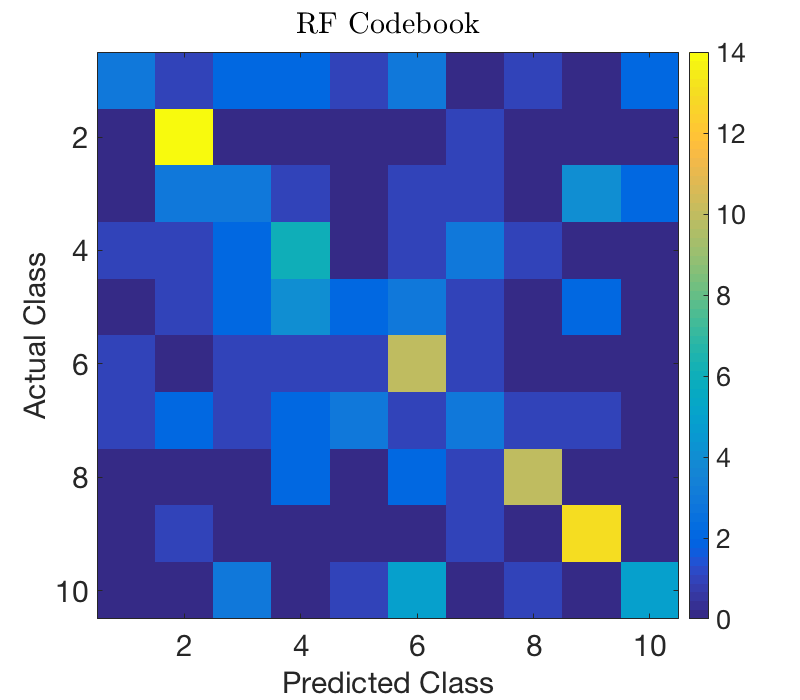
\includegraphics[width=\textwidth]{img/rfrf26}
      \caption{2 trees, depth 6.}
      \label{fig:rfrf2}
    \end{subfigure}
    \\
    \begin{subfigure}{0.45\linewidth}
      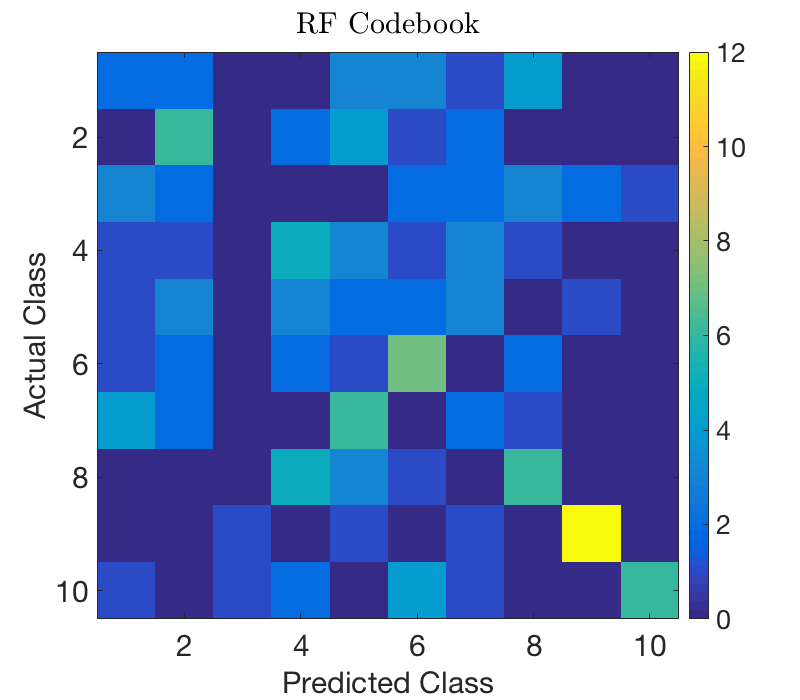
\includegraphics[width=\textwidth]{img/rfrf62}
      \caption{6 trees, depth 2.}
      \label{fig:rfrf3}
    \end{subfigure}
    ~
    \begin{subfigure}{0.45\linewidth}
      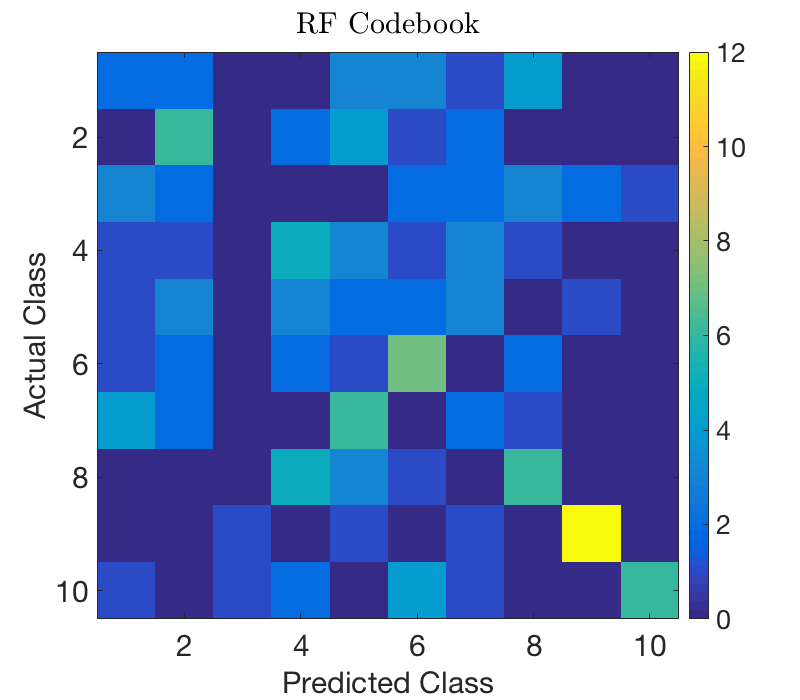
\includegraphics[width=\textwidth]{img/rfrf66}
      \caption{6 trees, depth 6.}
      \label{fig:rfrf4}
    \end{subfigure}

  \caption{Confusion Matrices with RF codebook and RF classifier.}
  \label{fig:rfrf}
\end{figure}

\end{document}
